\documentclass[12pt]{article}
% default article class values
% textwidth = 0.7 paperwidth = 1675.8pt
% textheight = 0.7 paperheight = 4788pt
% left = right = .15 paperwidth = 359.1pt
% top = (2/5)(.3 paperheight) = 820.8pt
% bottom = (3/5)(.3 paperheight) = 1231.2pt
\usepackage[% default layout
    a4paper, %showframe,
    left=0.15\paperwidth,
    %textwidth=0.55\paperwidth,
    textwidth=0.7\paperwidth,
    top=0.1\paperheight,
    bottom=0.1\paperheight,
    marginparwidth=0.2\paperwidth,
    marginparsep=15pt]{geometry}
\setlength\parindent{0mm}%

%%%%%%%%%%%%%%%%%%%%%%%%%%%%%%%%%%%%%%%%%%%%%%%%%%%%%%%%%
%% Packages
\usepackage{amsmath,amssymb}% AMS symbols and environments
\usepackage{mathtools}% More math symbols and environments
\usepackage[main=english]{babel}% Correct hyphenation
\usepackage{booktabs}% Nicer tables
\usepackage{caption}% Nicer captions
\captionsetup{labelfont=bf,textfont=bf}
\usepackage{xcolor}% Colours in text
\usepackage{graphicx}% 
\usepackage{pdfpages}% \includepdf
\usepackage[section]{placeins}%
\usepackage{sidenotes}% margin notes
\PassOptionsToPackage{hyphens}{url}\usepackage[
            breaklinks=true,colorlinks=true]{hyperref}
\usepackage{verbatim}% comment environment
%%%%%%%%%%%%%%%%%%%%%%%%%%%%%%%%%%%%%%%%%%%%%%%%%%%%%%%%%


%%%%%%%%%%%%%%%%%%%%%%%%%%%%%%%%%%%%%%%%%%%%%%%%%%%%%%%%%
%% Align table/figure top
\makeatletter
\setlength{\@fptop}{0pt}
\makeatother
%%%%%%%%%%%%%%%%%%%%%%%%%%%%%%%%%%%%%%%%%%%%%%%%%%%%%%%%%


\author{Dr Patrick Toche}
\title{Plot with R and ggplot2}
\date{Several plots with varying degrees of customization.}

\begin{document}
\maketitle

\begin{figure}[!htb]
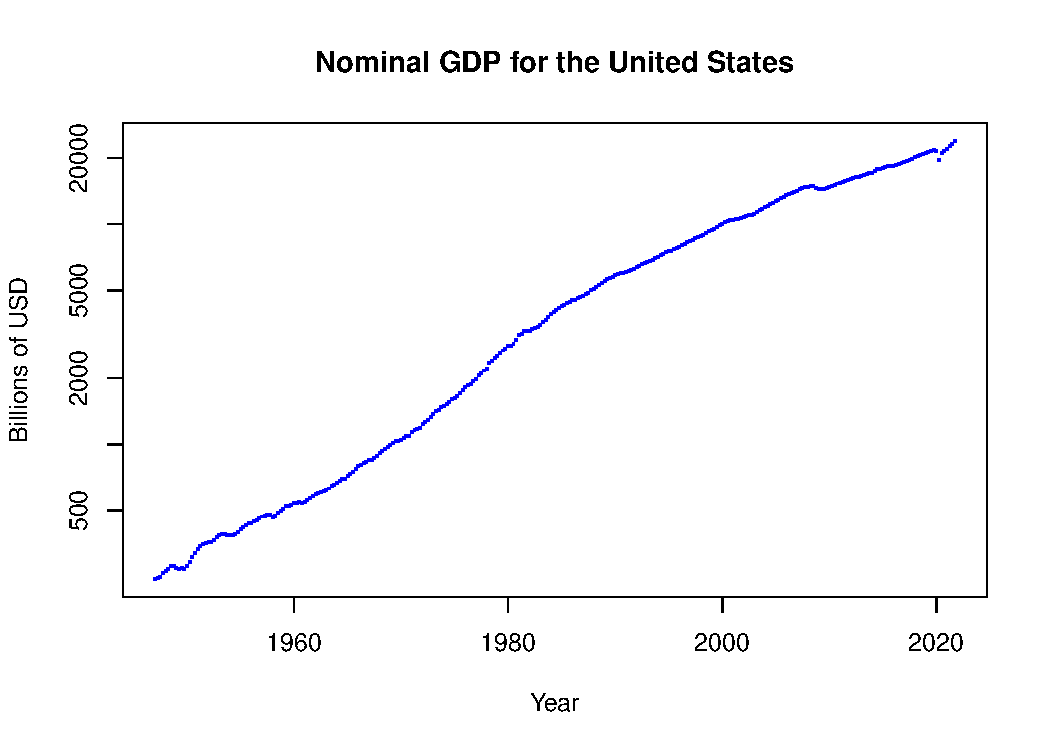
\includegraphics[height=0.4\textheight]{plot-gdp-nominal-logscale-basic}
\caption*{Basic R Plot}
\end{figure}

\begin{figure}[!htb]
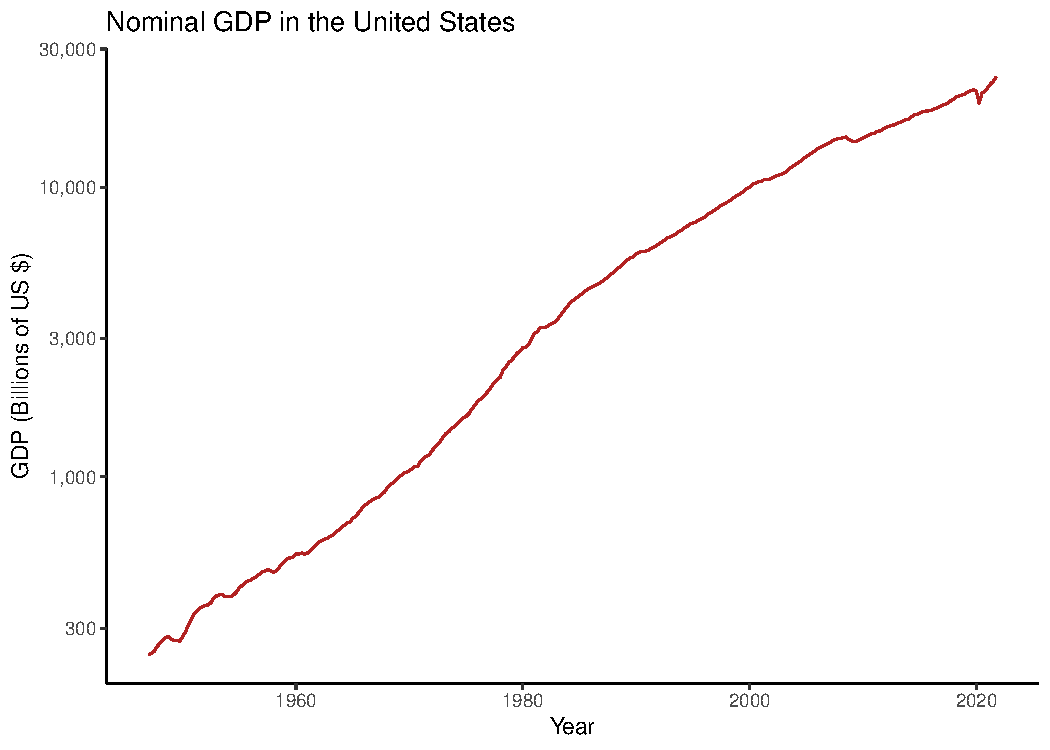
\includegraphics[height=0.4\textheight]{plot-gdp-nominal-logscale-ggplot}
\caption*{Basic ggplot Plot}
\end{figure}

\begin{figure}[!htb]
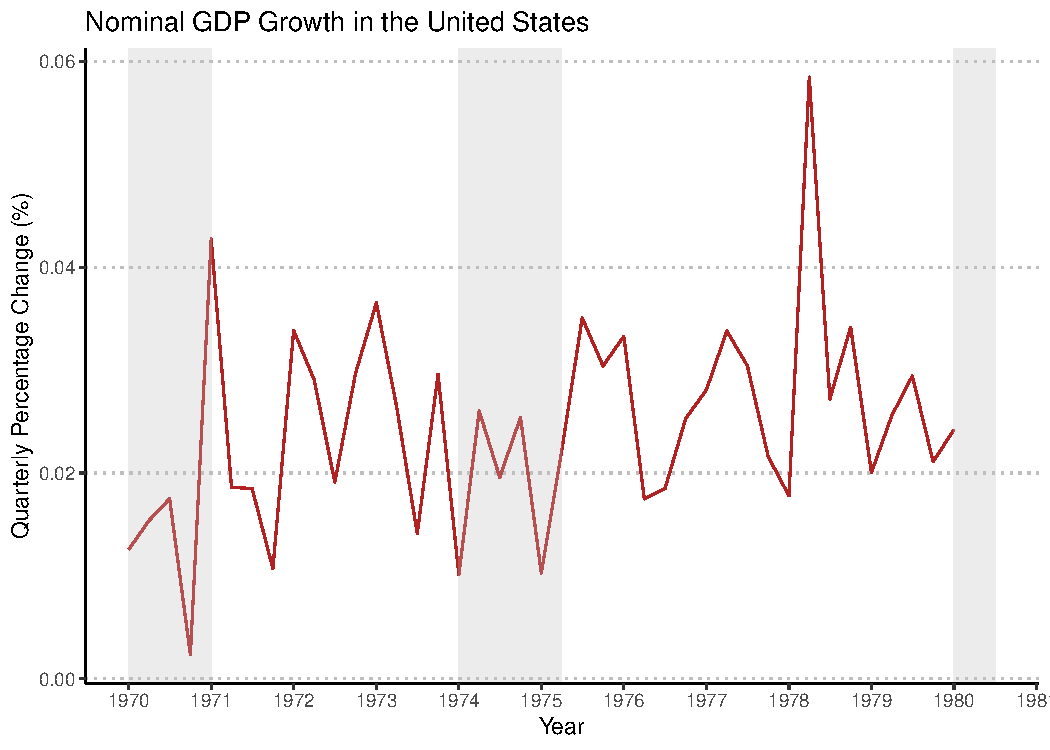
\includegraphics[height=0.4\textheight]{plot-gdp-nominal-growth-q-nber}
\caption*{The quarterly growth rate is very volatile}
\end{figure}

\begin{figure}[!htb]
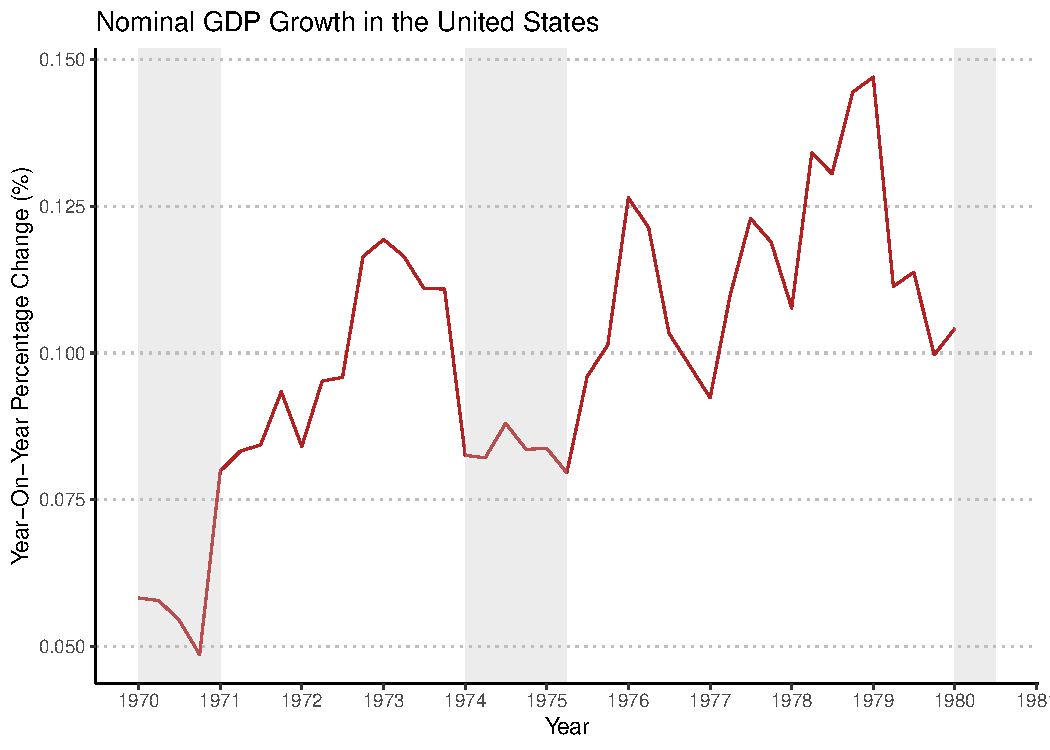
\includegraphics[height=0.4\textheight]{plot-gdp-nominal-growth-yoy-nber}
\caption*{The year-on-year growth rate is less volatile than the quarterly rate}
\end{figure}

\begin{figure}[!htb]
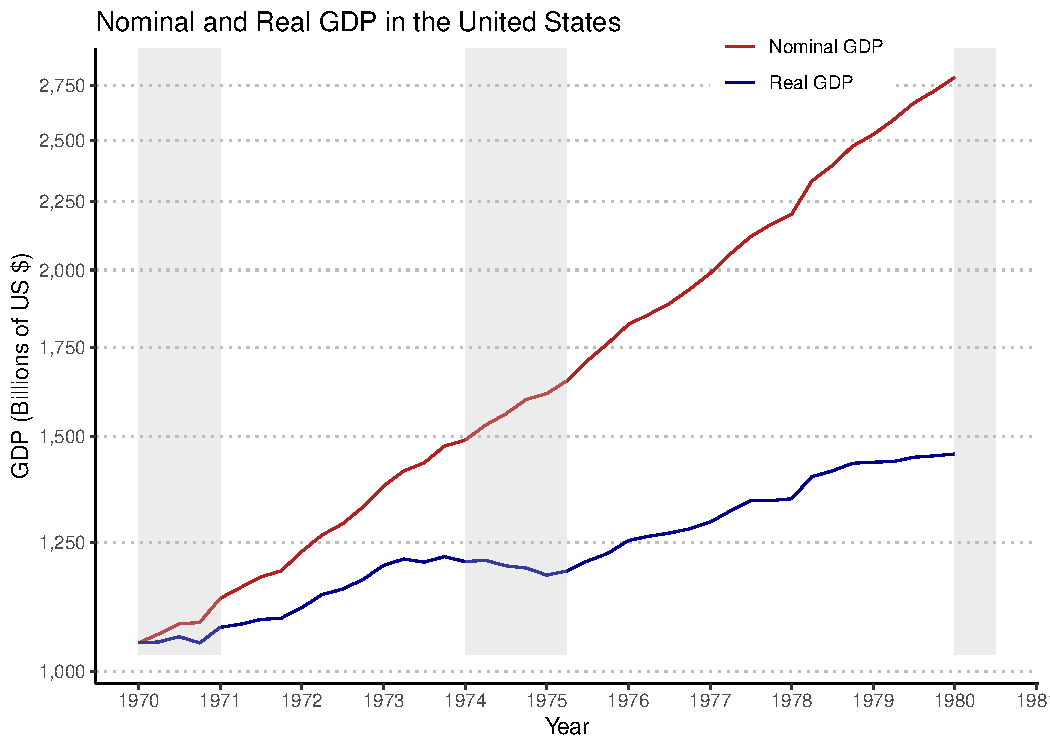
\includegraphics[height=0.4\textheight]{plot-gdp-nominal-real-logscale-nber}
\caption*{Much of the growth in nominal GDP is inflation}
\end{figure}

\end{document}
